% Basic Beamer template
% Compile with: ./in-docker pdflatex presentation.tex

\documentclass{beamer}

% Theme - you can change this
\usetheme{Madrid}
\usecolortheme{default}

% For including graphics
\usepackage{graphicx}

% T1 font encoding: needed for special characters (German quotes, µ, accents)
\usepackage[T1]{fontenc}

% For strikethrough text (\sout)
\usepackage[normalem]{ulem}

% Title page info
\title{XTC next steps}
\subtitle{Using XTC in real life problems}
\author{Sylvain Noiry}
\institute{Inria, Kalray}
\date{\today}

\begin{document}

% Title frame
\begin{frame}
    \titlepage
\end{frame}

% Section 1
\section{Introduction}
\begin{frame}{Introduction}
    \begin{columns}[T]
        \begin{column}{0.35\textwidth}
            \begin{center}
                
\includegraphics[width=0.9\textwidth]{figures/yoda.png}
            \end{center}
        \end{column}
        \begin{column}{0.6\textwidth}
            \begin{quote}
                \itshape
                ``Know XTC, the world must. Advert it with new use cases, you will.''
            \end{quote}
            \begin{flushright}
                \onslide<2->{--- Albert Cohen}
            \end{flushright}
        \end{column}
    \end{columns}
\end{frame}


% Outline frame
%\begin{frame}{Outline}
%    \tableofcontents
%\end{frame}

% Section 1
\section{dram}
\begin{frame}{DRAM crisis}
    \begin{columns}[T]
        \begin{column}{0.42\textwidth}
            Sam Altman needs your DRAM
            \begin{itemize}
		\item HBM, GDDR of course
                \item DDR5, DDR4, DDR3... also
                \item SRAM why not
                \item ...
            \end{itemize}
        \end{column}
        \begin{column}{0.22\textwidth}
            \vspace*{3cm}
            \begin{center}
                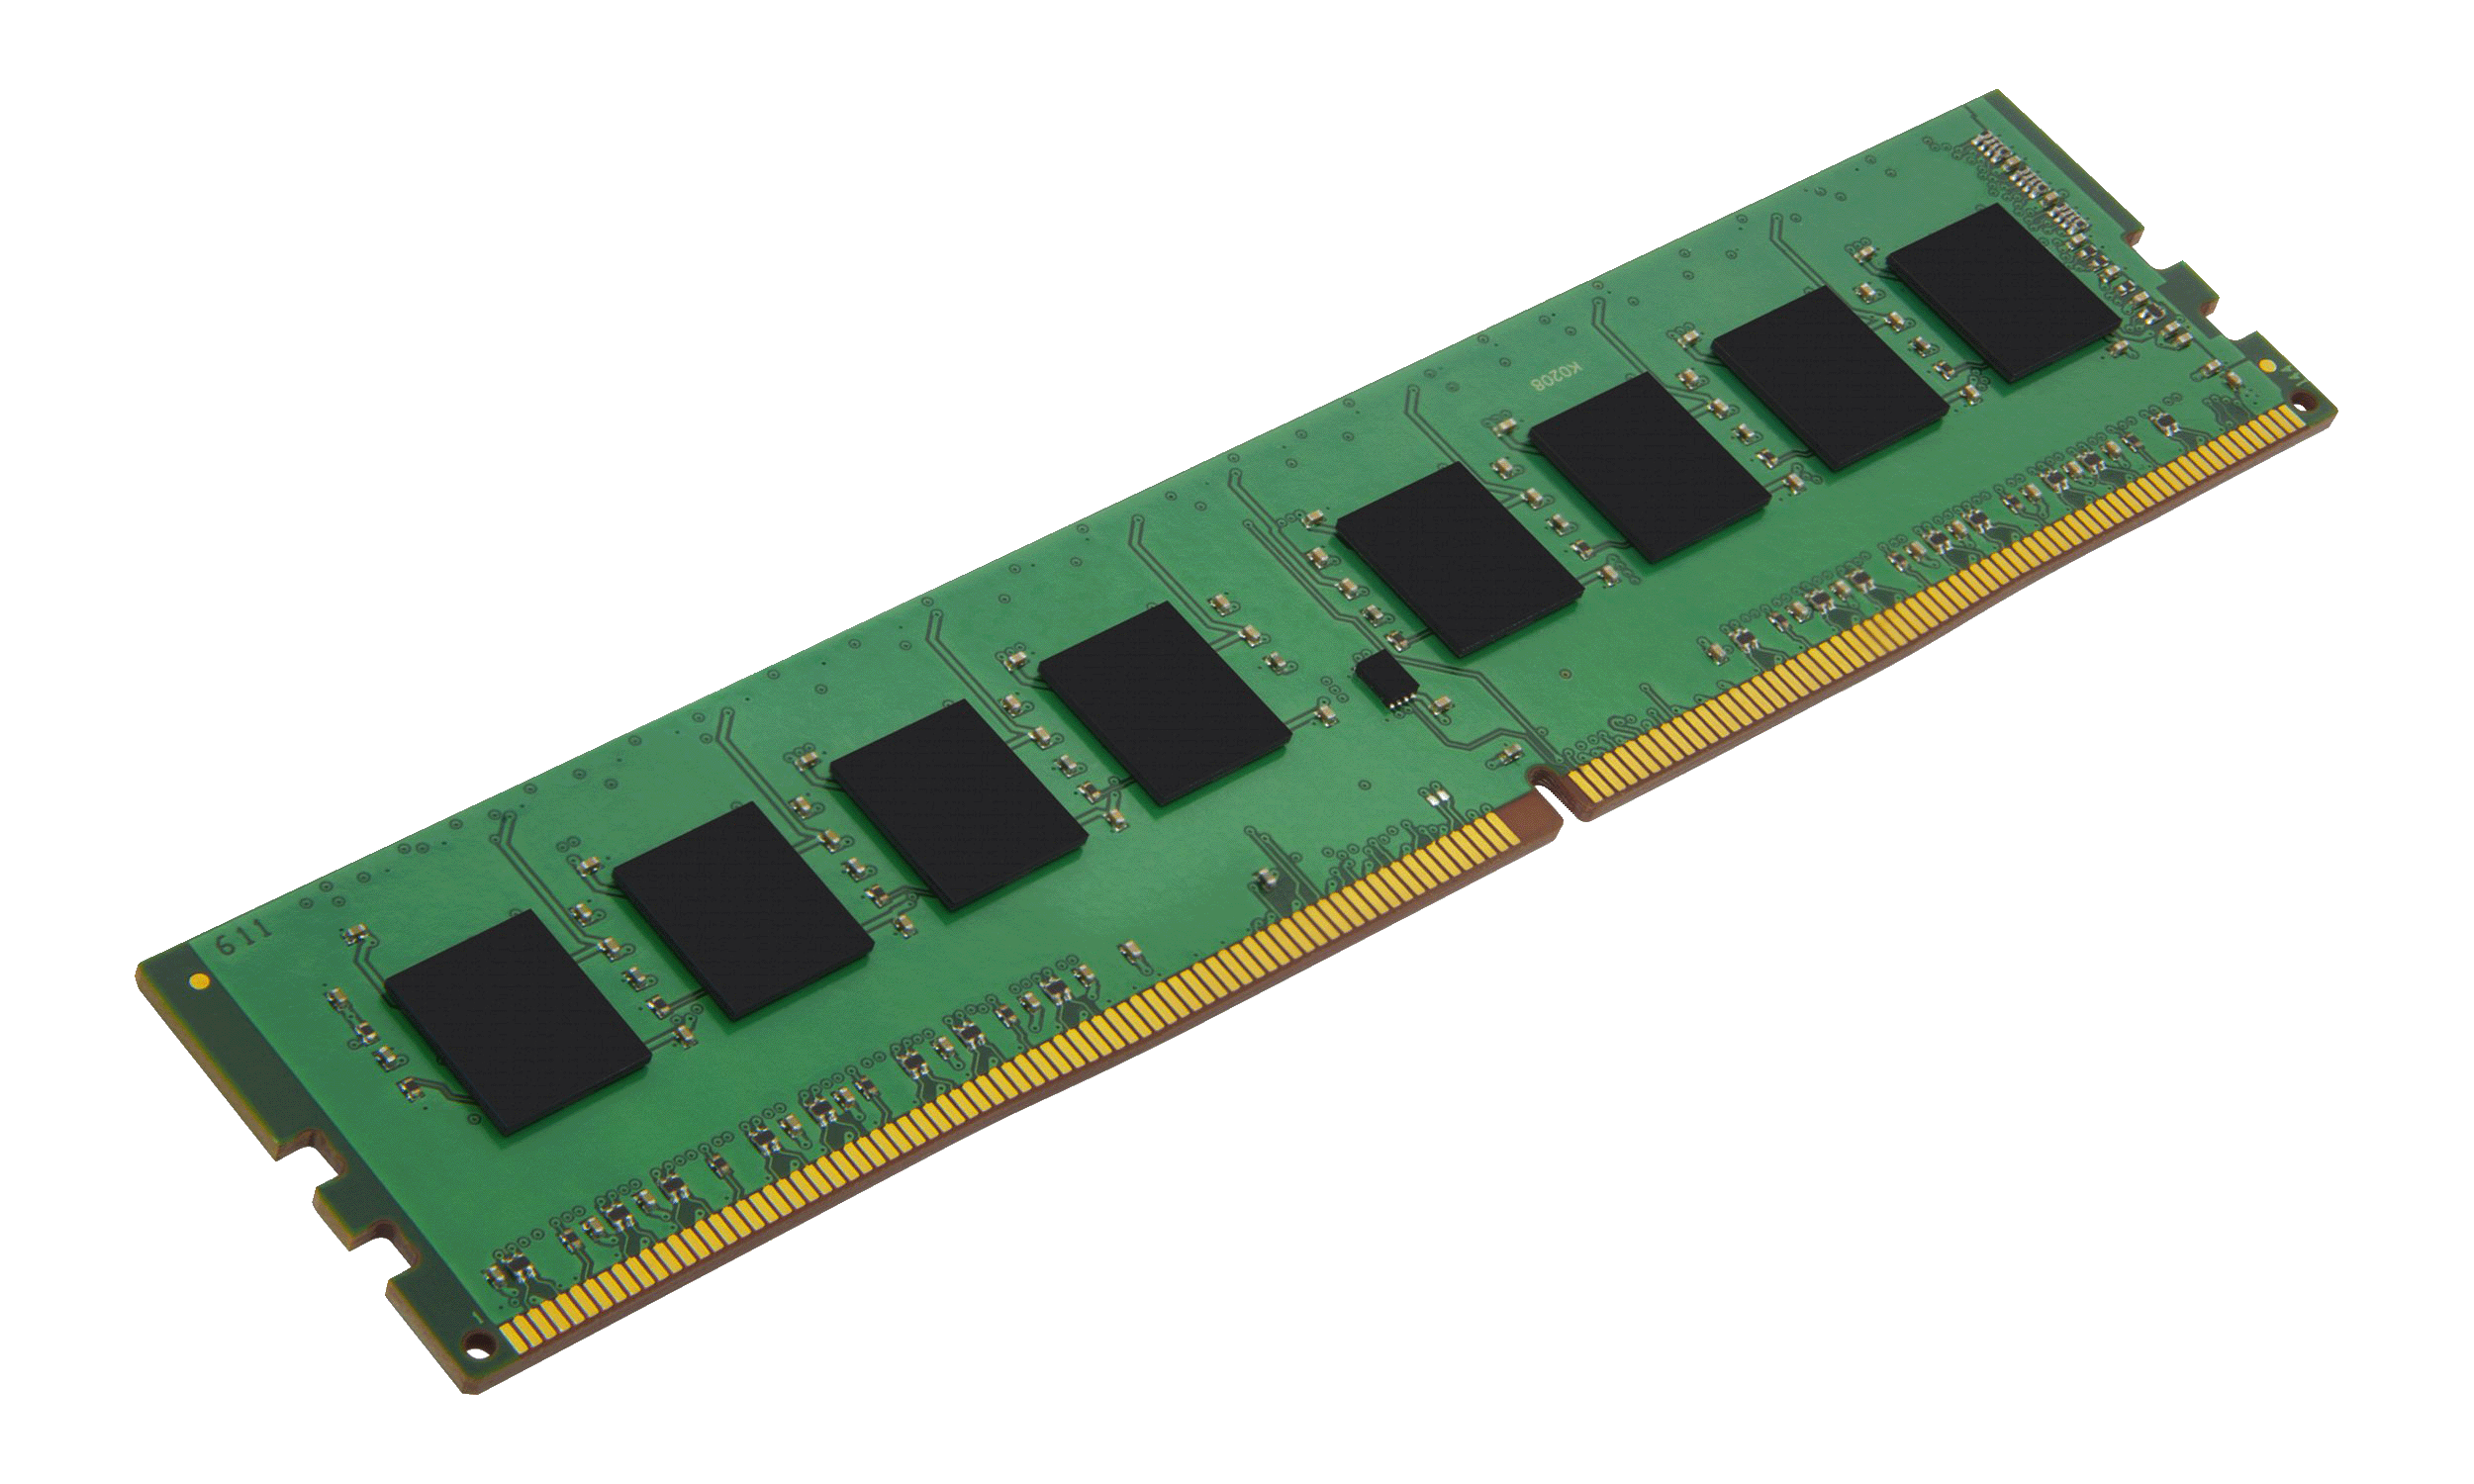
\includegraphics[width=\textwidth]{figures/ram.png}
            \end{center}
        \end{column}
        \begin{column}{0.33\textwidth}
            \begin{center}
                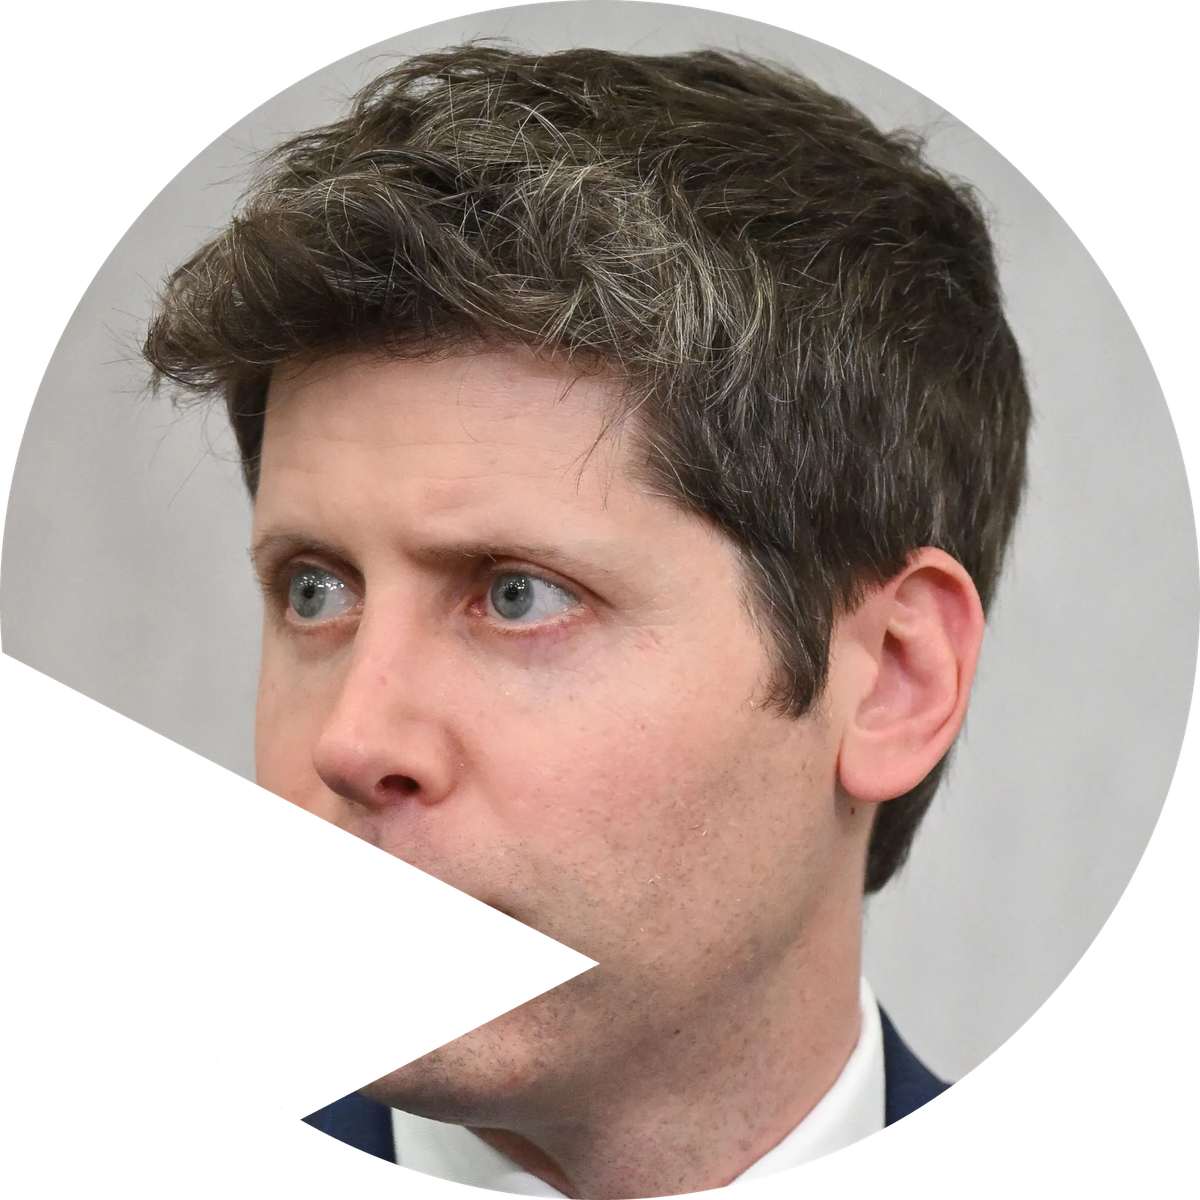
\includegraphics[width=\textwidth]{figures/pacman_sam_altman.png}
            \end{center}
        \end{column}
    \end{columns}
	\onslide<2->{$\rightarrow$ Sam altman is probably right, we need to learn how to use less RAM, but still run Matmuls !}
\end{frame}

\section{solution}
\begin{frame}{A solution exists !}
    \begin{itemize}
        \item Low power
	\item Cheap
        \item Easy schedules for XTC
	\item Easy reverse engineering (for Alban)
	\item Well documented
    \end{itemize}
\end{frame}

% Section 2
\section{z80}
\begin{frame}{Zilog Z80 !}
    
    \begin{center}
        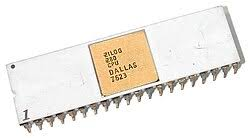
\includegraphics[width=0.6\textwidth]{figures/z80.png}
    \end{center}
    
    %\begin{block}{}
    %    This is an important result.
    %\end{block}
    %
    %\begin{alertblock}{Warning}
    %    This is something to be careful about.
    %\end{alertblock}
    %
    %\begin{exampleblock}{Example}
    %    This is an example.
    %\end{exampleblock}
\end{frame}

\begin{frame}{Zilog Z80 !}
    
	8500 transistors in 4µm (no competition with Sam Altmam)
    \begin{center}
        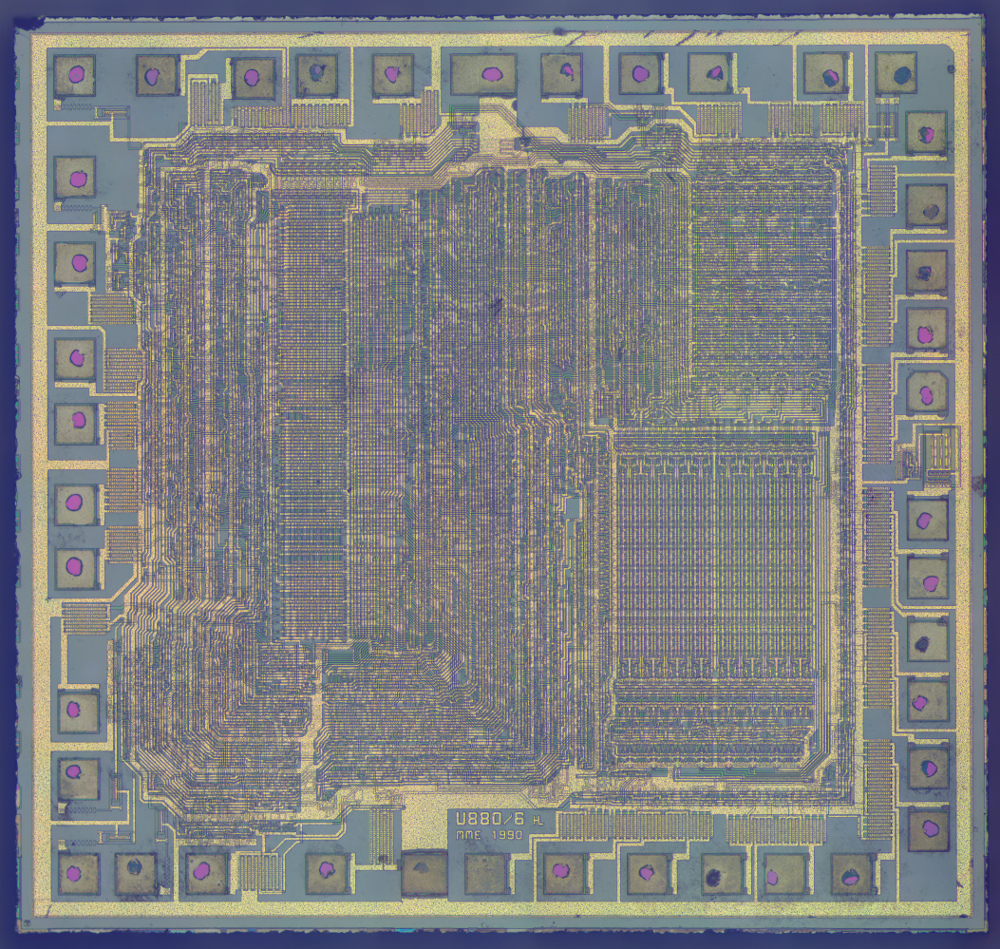
\includegraphics[width=0.5\textwidth]{figures/z80_ussr.jpg}
    \end{center}
    \small
	Even USSR could make it \textit{(KR1858VM1 from VEB Mikroelektronik „Karl Marx“)}

    %\begin{block}{}
    %    This is an important result.
    %\end{block}
    %
    %\begin{alertblock}{Warning}
    %    This is something to be careful about.
    %\end{alertblock}
    %
    %\begin{exampleblock}{Example}
    %    This is an example.
    %\end{exampleblock}
\end{frame}

\section{z80reverse}
\begin{frame}{Reverse engineering is easy !}
    \begin{center}
        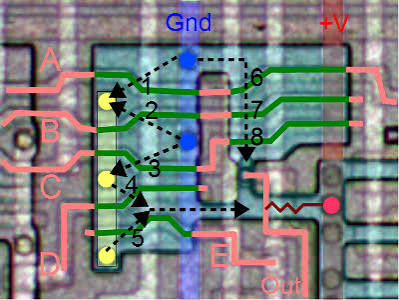
\includegraphics[width=0.6\textwidth]{figures/transistors.png}
    \end{center}
\end{frame}

\begin{frame}{Reverse engineering is easy !}
    \begin{center}
        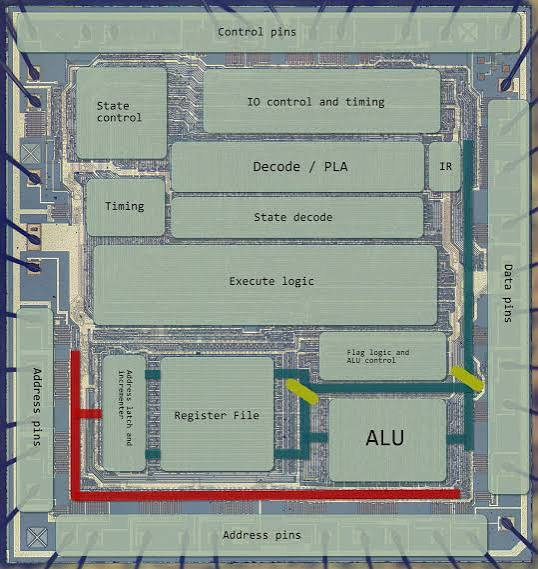
\includegraphics[width=0.6\textwidth]{figures/die_shot_annotation.png}
    \end{center}
\end{frame}

\section{z80ram}
\begin{frame}{A few KB of DRAM is enough}
    \textbf{Can (almost) be made in a garage !}
    \begin{center}
        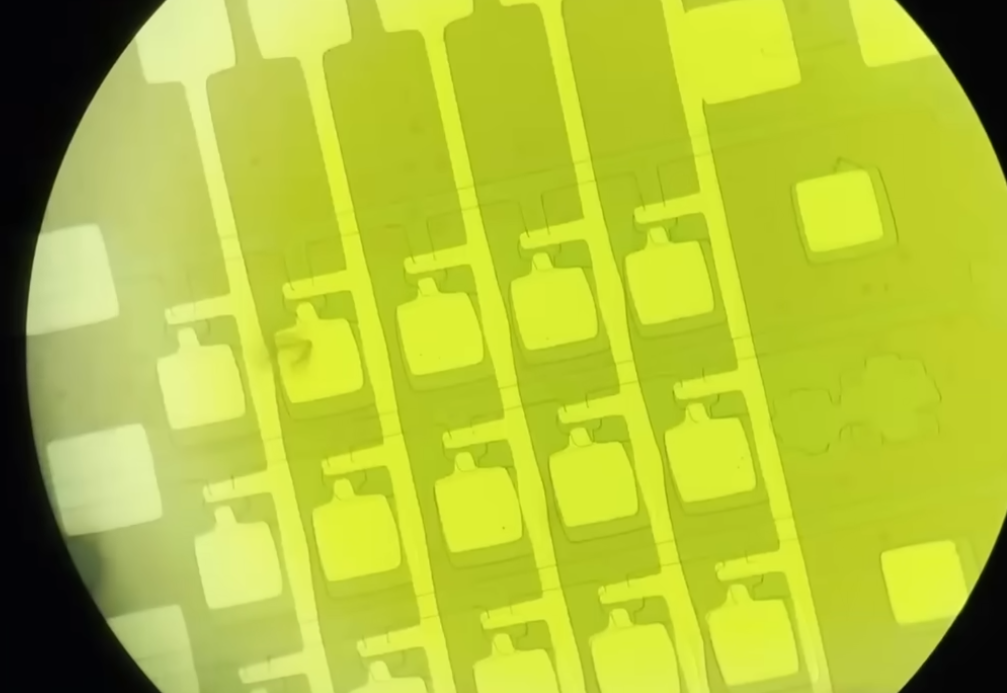
\includegraphics[width=0.6\textwidth]{figures/garage_dram.png}
	    \url{https://www.youtube.com/watch?v=h6GWikWlAQA}
    \end{center}
\end{frame}

\section{schedules}
\begin{frame}{Schedules are super easy !}
    \Large
    \begin{itemize}
	\onslide<2->{\item \sout{Out-Of-Order} $\rightarrow$ Over-engineered}
	\onslide<3->{\item \sout{Superscalar} $\rightarrow$ Makes life simpler}
	\onslide<4->{\item \sout{Cache} $\rightarrow$ Single level tiling}
	\onslide<5->{\item \sout{Vectorization} $\rightarrow$ Scalar}
	\onslide<6->{\item \sout{Strided access} $\rightarrow$ No packing/padding}
	\onslide<7->{\item \sout{Multicore} $\rightarrow$ No parallelism}
	\onslide<8->{\item \sout{Floating point}}
    \end{itemize}
\end{frame}

\begin{frame}[fragile]
    \begin{semiverbatim}
sch.strip_mine("i", \{"i1": 4\})
sch.strip_mine("j", \{"j1": 1\})
sch.interchange(["k", "i", "j", "i1", "j1"])
    \end{semiverbatim}
\end{frame}

\begin{frame}
	\Large
	\begin{center}
		DEMO !
	\end{center}
\end{frame}


% Section 3
\section{Conclusion}
\begin{frame}{Conclusion}
	\Large
	$\rightarrow$ Let's start the real presentation
\end{frame}

\end{document}
